\chapter{\ifproject%
\ifenglish Experimentation and Results\else การทดลองและผลลัพธ์\fi
\else%
\ifenglish System Evaluation\else การประเมินระบบ\fi
\fi}
\hspace{10mm} เนื่องจากมีการนำความรู้เรื่อง Computer Vision มาใช้เกี่ยวกับการทำ Object detection จึงได้มีการศึกษา model และ library
ของ OpenCV ที่มีให้ทดลองใช้งาน เพื่อเพิ่มความเข้าใจและเลือกใช้ได้อย่างเหมาะสม โดยนำภาพบางส่วนจากการถ่ายรูปสถานที่จริงด้วยกล้องโทรศัพท์มือถือคือบริเวณชั้น 2
ของสำนักหอสมุดมหาวิทยาลัยเชียงใหม่มาทำการทดสอบจึงมีการทดลองทั้งหมด 3 ครั้ง
\begin{figure}[ht]
    \centering
    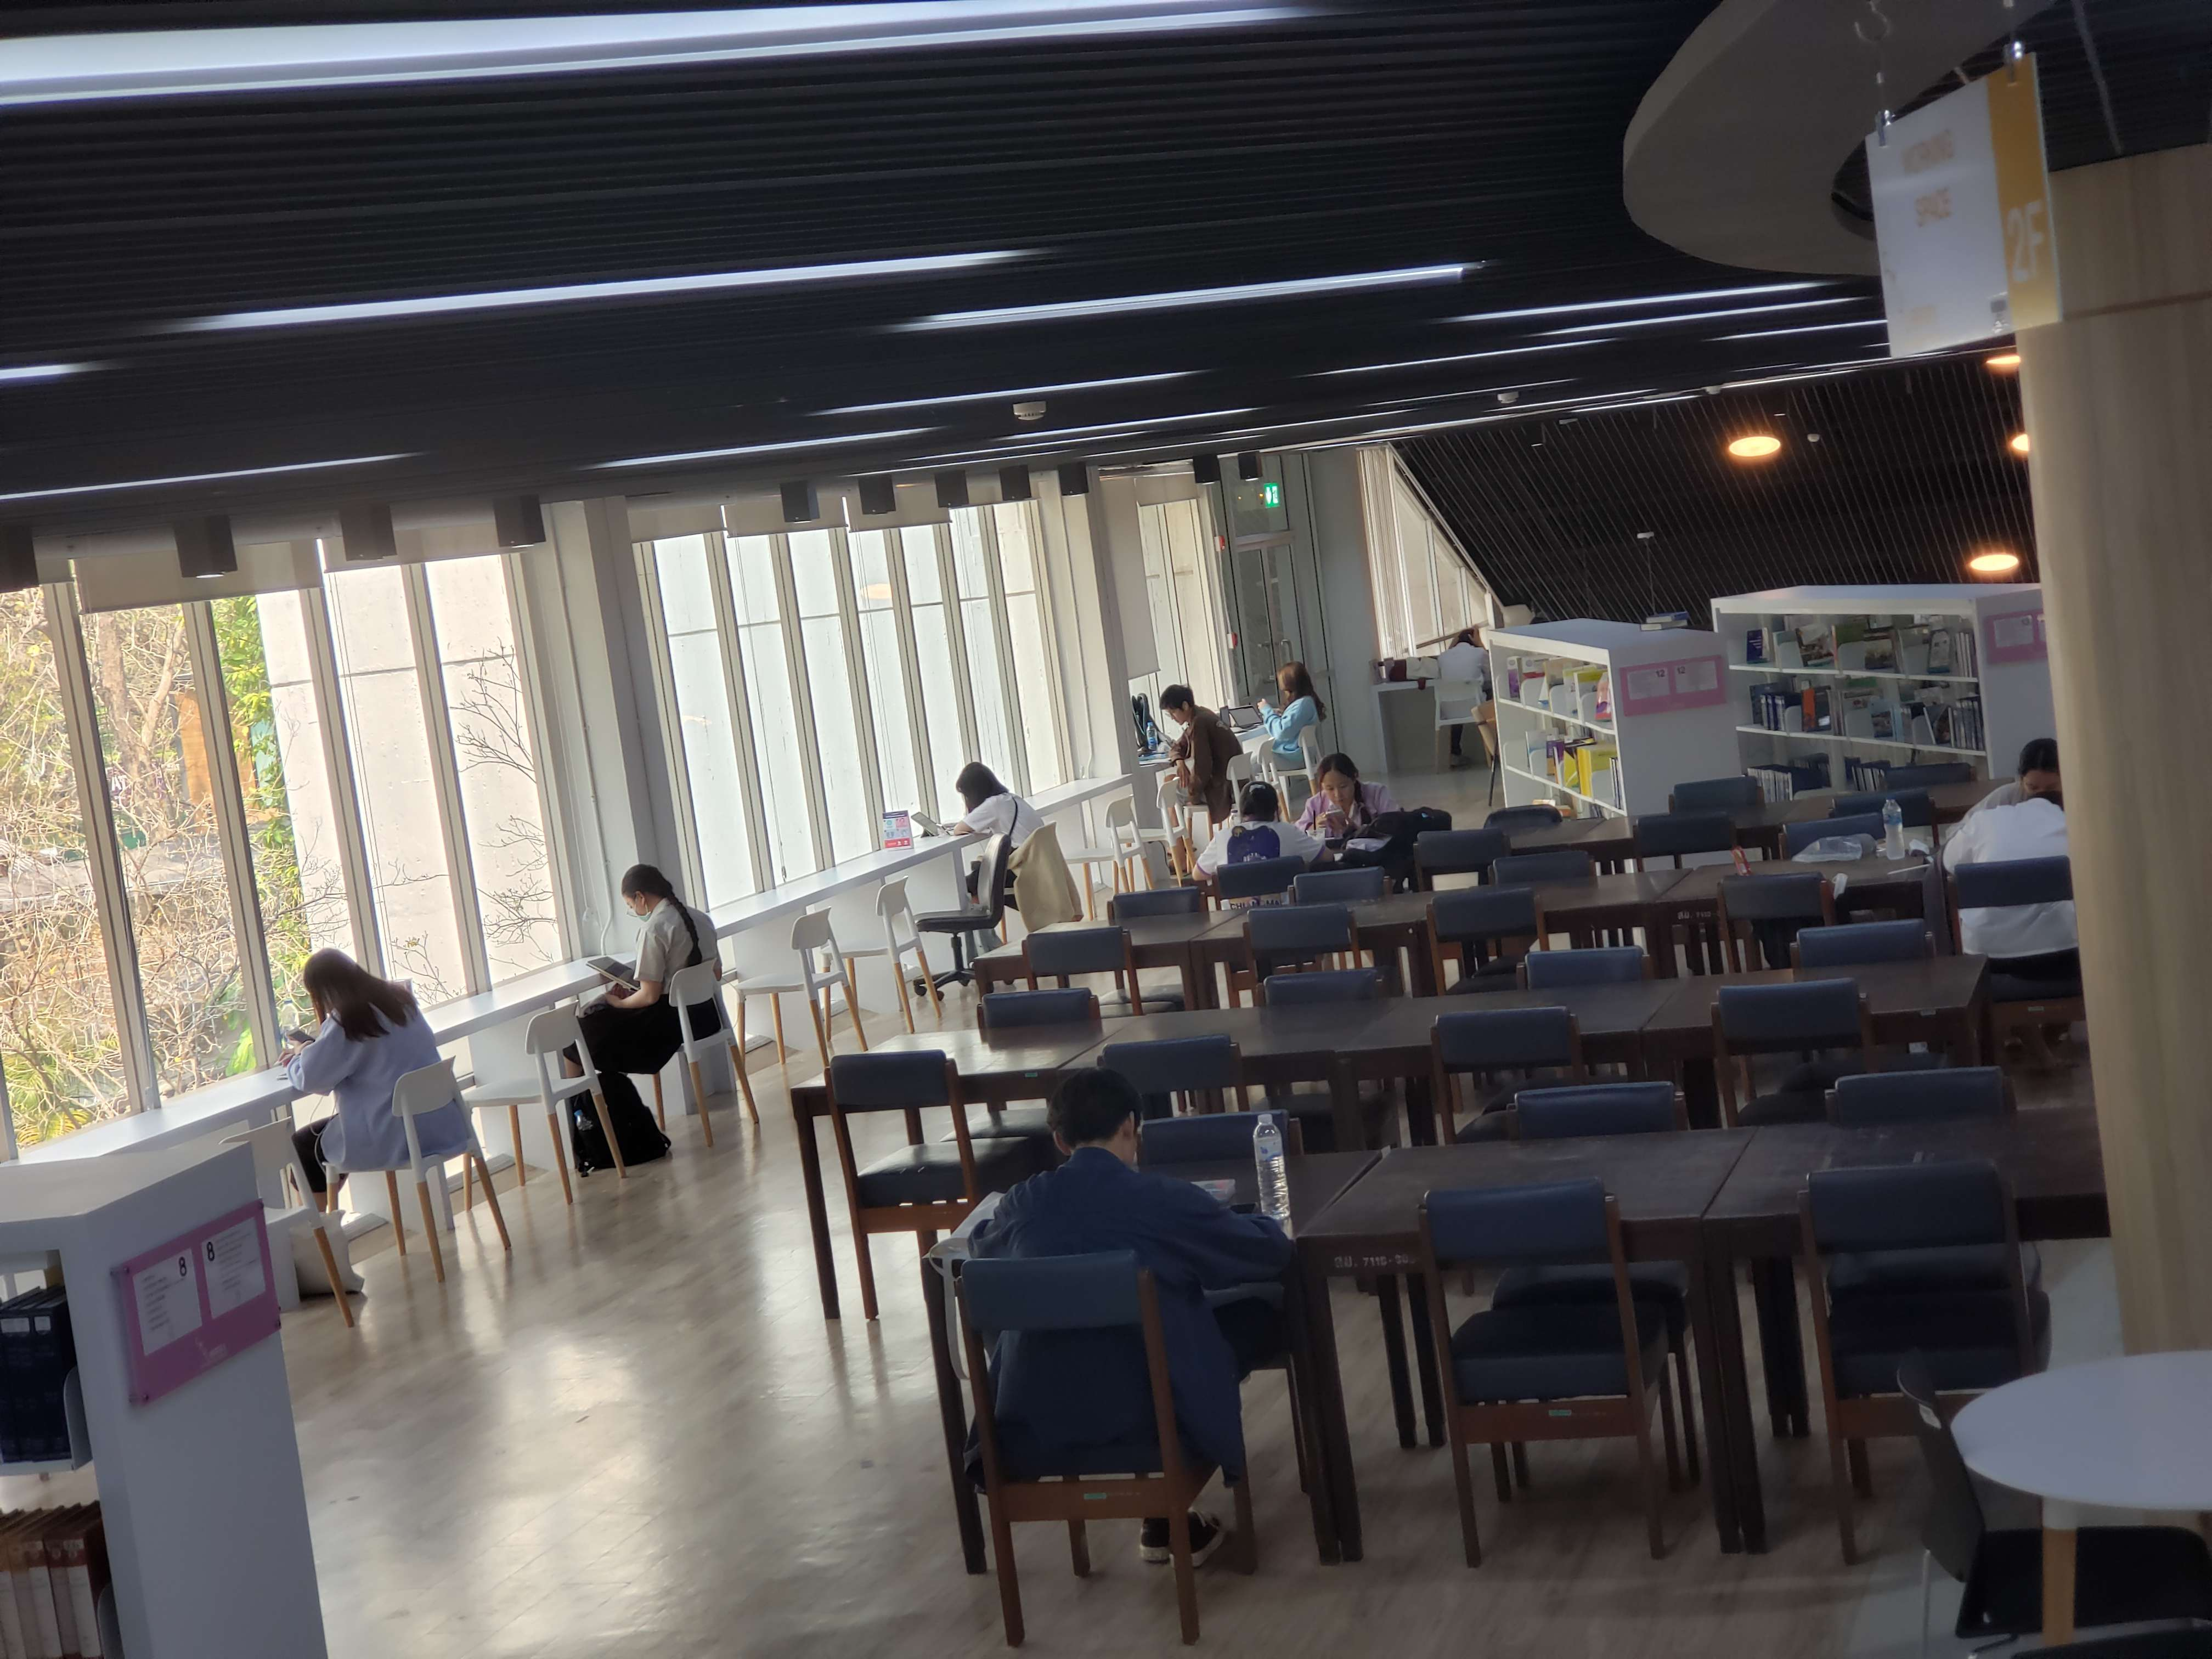
\includegraphics[scale=0.07]{images/cam2-2.jpg}
    \caption[camera]{ภาพจากกล้องโทรศัพท์มือถือ}
    \label{fig:camera}
\end{figure}
\newpage
\section{การทดลองครั้งที่ 1 โดยใช้ OpenCV with HOG descriptor}
<<<<<<< HEAD

=======
>>>>>>> 4ea343bead47c8936409792963f802ead21bafed
\hspace{10mm}HOG (Histograms of Oriented Gradients) descriptor เป็น library ที่ทาง OpenCV มีให้ใช้
ซึ่งใช้ร่วมกับ SVM Classifier ที่ได้รับการ train มาแล้วจาก cv2.HOGDescriptor\textunderscore getDefaultPeopleDetector()
ในการจำแนกว่าเป็นคนหรือไม่ใช่คน

\begin{figure}[ht]
    \centering
    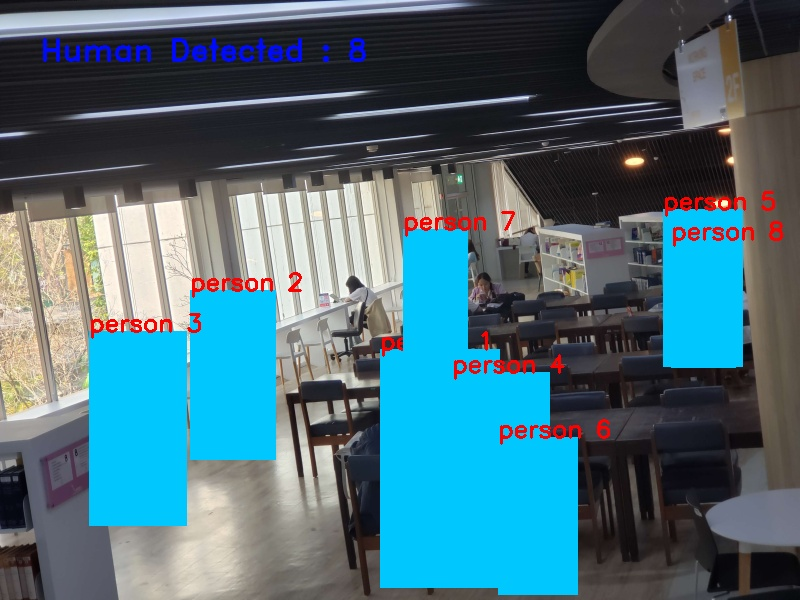
\includegraphics[scale=0.35]{images/hog_output.jpg}
    \caption[output 1]{output ของการทดลองครั้งที่ 1}
    \label{fig:output1}
<<<<<<< HEAD
\end{figure}

ผลลัพธ์ที่ได้คือสามารถตรวจจับคนในภาพได้จำนวน 8 คน ซึ่งได้จำนวนมากกว่าความเป็นจริง และตรวจจับได้ในส่วนที่ไม่ใช่คนอีกด้วย
=======
    \end{figure}
>>>>>>> 4ea343bead47c8936409792963f802ead21bafed

\hspace{10mm} ผลลัพธ์ที่ได้คือสามารถตรวจจับคนในภาพได้จำนวน 8 คน ซึ่งได้จำนวนมากกว่าความเป็นจริง และตรวจจับได้ในส่วนที่ไม่ใช่คนอีกด้วย
\newpage
\section{การทดลองครั้งที่ 2 โดยใช้ OpenCV with Detect common object library}
\hspace{10mm}Detect common object library เป็น library ที่ทาง OpenCV มีให้ใช้ ซึ่งสามารถตรวจจับวัตถุพื้นฐานได้จาก model YOLOv3 แต่ในการทดลองนี้จะเลือกให้ตรวจจับเฉพาะคนเท่านั้น
\begin{figure}[ht]
    \centering
    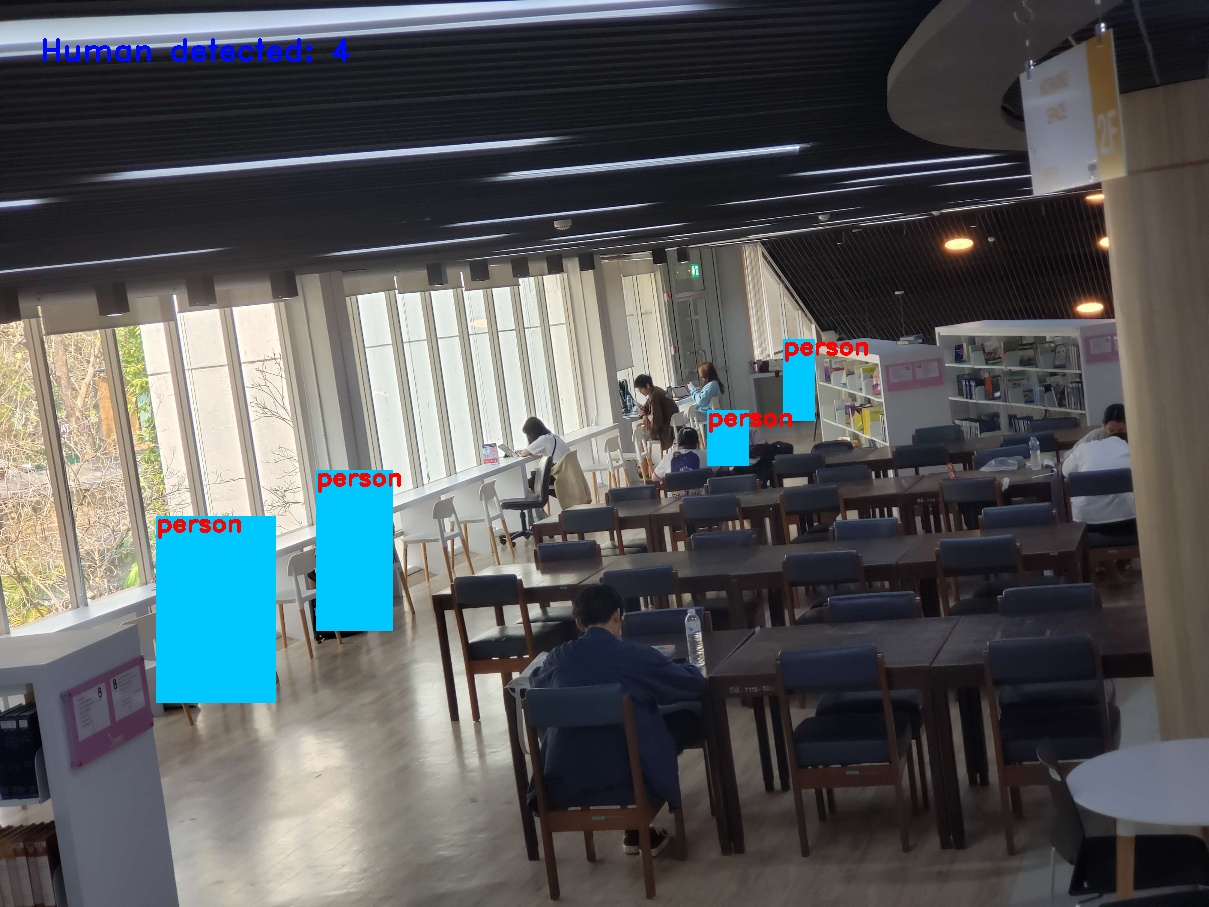
\includegraphics[scale=0.25]{images/cvlib_output.jpg}
    \caption[output 2]{output ของการทดลองครั้งที่ 2}
    \label{fig:output2}
\end{figure}

ผลลัพธ์ที่ได้คือสามารถตรวจจับคนในภาพได้จำนวน 4 คน ซึ่งได้จำนวนน้อยกว่าความเป็นจริง
\newpage
\section{การทดลองครั้งที่ 3 โดยใช้ OpenCV DNN with TensorFlow}
\hspace{10mm} OpenCV มี DNN (Deep Neural Network) module ที่สามารถนำ model จาก TensorFlow มาใช้ได้ โดยการทดลองนี้ได้เลือก model MobileNet-SSD v2 ที่มีความนิยมมาใช้

\begin{figure}[ht]
    \centering
    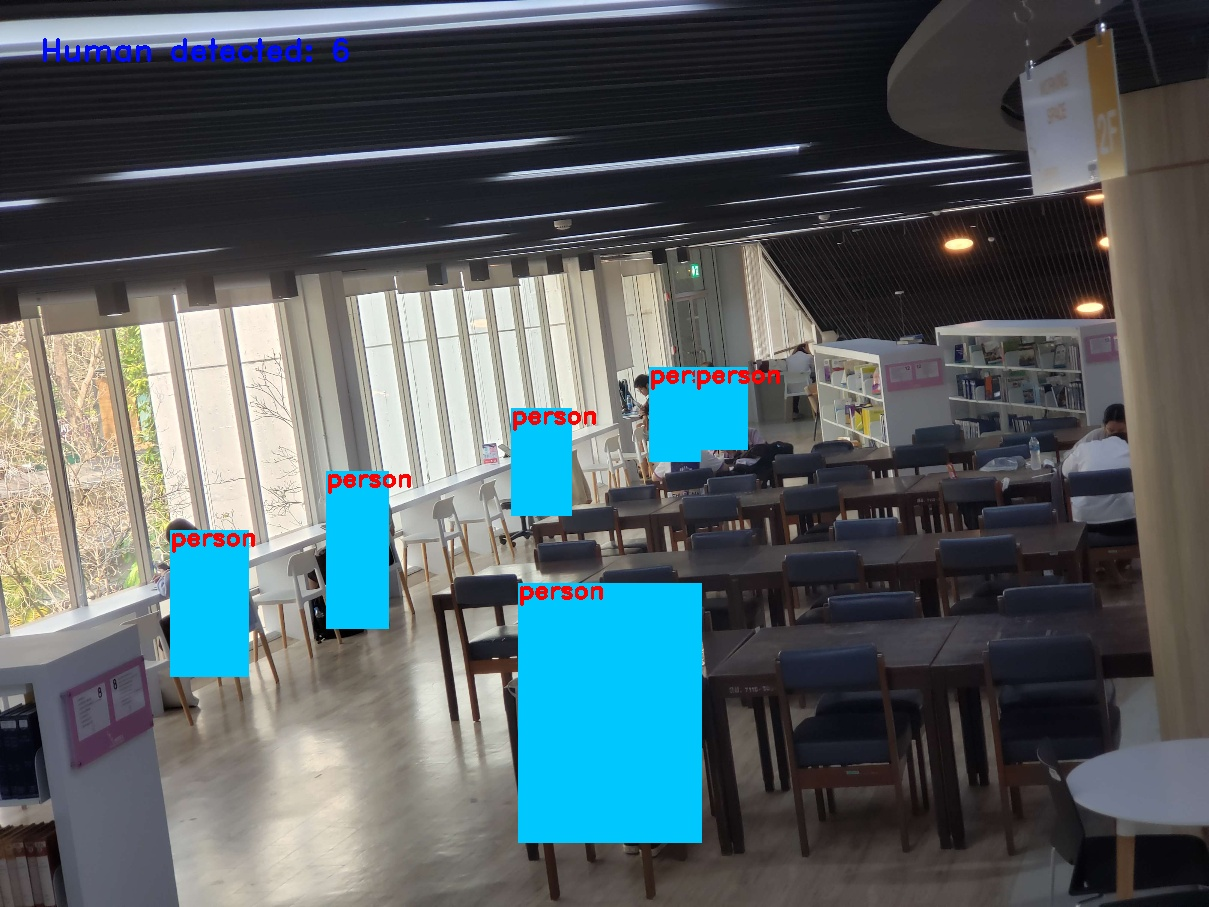
\includegraphics[scale=0.25]{images/dnn_output.jpg}
    \caption[output 3]{output ของการทดลองครั้งที่ 3}
    \label{fig:output3}
\end{figure}
ผลลัพธ์ที่ได้คือสามารถตรวจจับคนในภาพได้จำนวน 6 คน ซึ่งได้จำนวนน้อยกว่าความเป็นจริงเล็กน้อย มีความสามารถในการตรวจจับคนได้มากกว่าการทดลองครั้งที่ 2
\section{สรุปผลการทดลอง}
\hspace{10mm} จากผลการทดลองพบว่าการวิเคราะห์ผลของการทดลองครั้งที่ 3 โดยใช้ OpenCV DNN with TensorFlow ออกมาได้ค่อนข้างตรงที่สุด จึงคาดว่าจะใช้ model นี้ในการพัฒนาโครงงาน
และในส่วนของการที่วิเคราะห์ผลออกมาผิดพลาดอาจเป็นเพราะมุมกล้อง ค่าสี ค่าความอิ่มตัวของสี หรือความสว่างของภาพที่อาจส่งผลต่อการวิเคราะห์ของ model จึงจะต้องมีการทดลองในส่วนนี้ต่อไป